\documentclass[11pt,a4paper,titlepage,oneside]{report}
\usepackage{titling}
\usepackage{graphicx}
\usepackage{mathtools}
\usepackage{lmodern}
\usepackage{amsmath}
\usepackage{float}
\usepackage{subfig}
\usepackage{listings}
\usepackage[hidelinks]{hyperref}

\input{layout}

\title{Point cloud-based camera calibration}
\author{Stefan Eichenberger}
\date{July 2018}
\advisors{Marcus Hudritsch}
\department{TSM CPVR Lab}

\begin{document}
\maketitle

\begin{abstract}
To reconstruct the pose and position of a camera the intrinsic camera model must once be calculated. We show a method on how to calibrate a camera based on a pre-generated point cloud. This method makes camera calibration more user friendly for augmented reality applications where pre-generated point clouds can be used.
\end{abstract}

\section*{Executive Summary}
Augmented reality is a fast growing area in computer vision. New sensors and faster processors make this technology possible.\\\\
One application we can realize with augmented reality is the virtual construction of buildings. We can project the virtual building onto an image of the location where the building stood/will stand. To make this projection possible, we must know the location of the viewer and the properties of the camera. In this project, we focus on finding the properties of the camera. Finding these properties is called camera calibration. We try to find a novel method to calibrate a camera based on known points. We need to know the position of these points in the 3D world and the position of the points in the 2D image.\\\\
The here shown approach allows us to calibrate a camera just in place. Existing calibration processes require an image of a checkerboard. This approach isn't intuitive for end users.

\tableofcontents

\chapter{Introduction}
To build a new railway station, the city of Bern decided in the year 1865 to tear down the Christoffeltower. This building was the entrance to Bern through the city wall. Today the area around the railway station is heavily used by buses and cars. Therefore, it is impossible to rebuild the tower physically. Luckily we nowadays have the technology to create an illusion of such a building. The idea is to build a virtual Christoffeltower by using augmented reality on a smartphone (see figure \ref{fig:christoffeltower}).\\\\
\begin{figure}[H]
  \begin{center}
		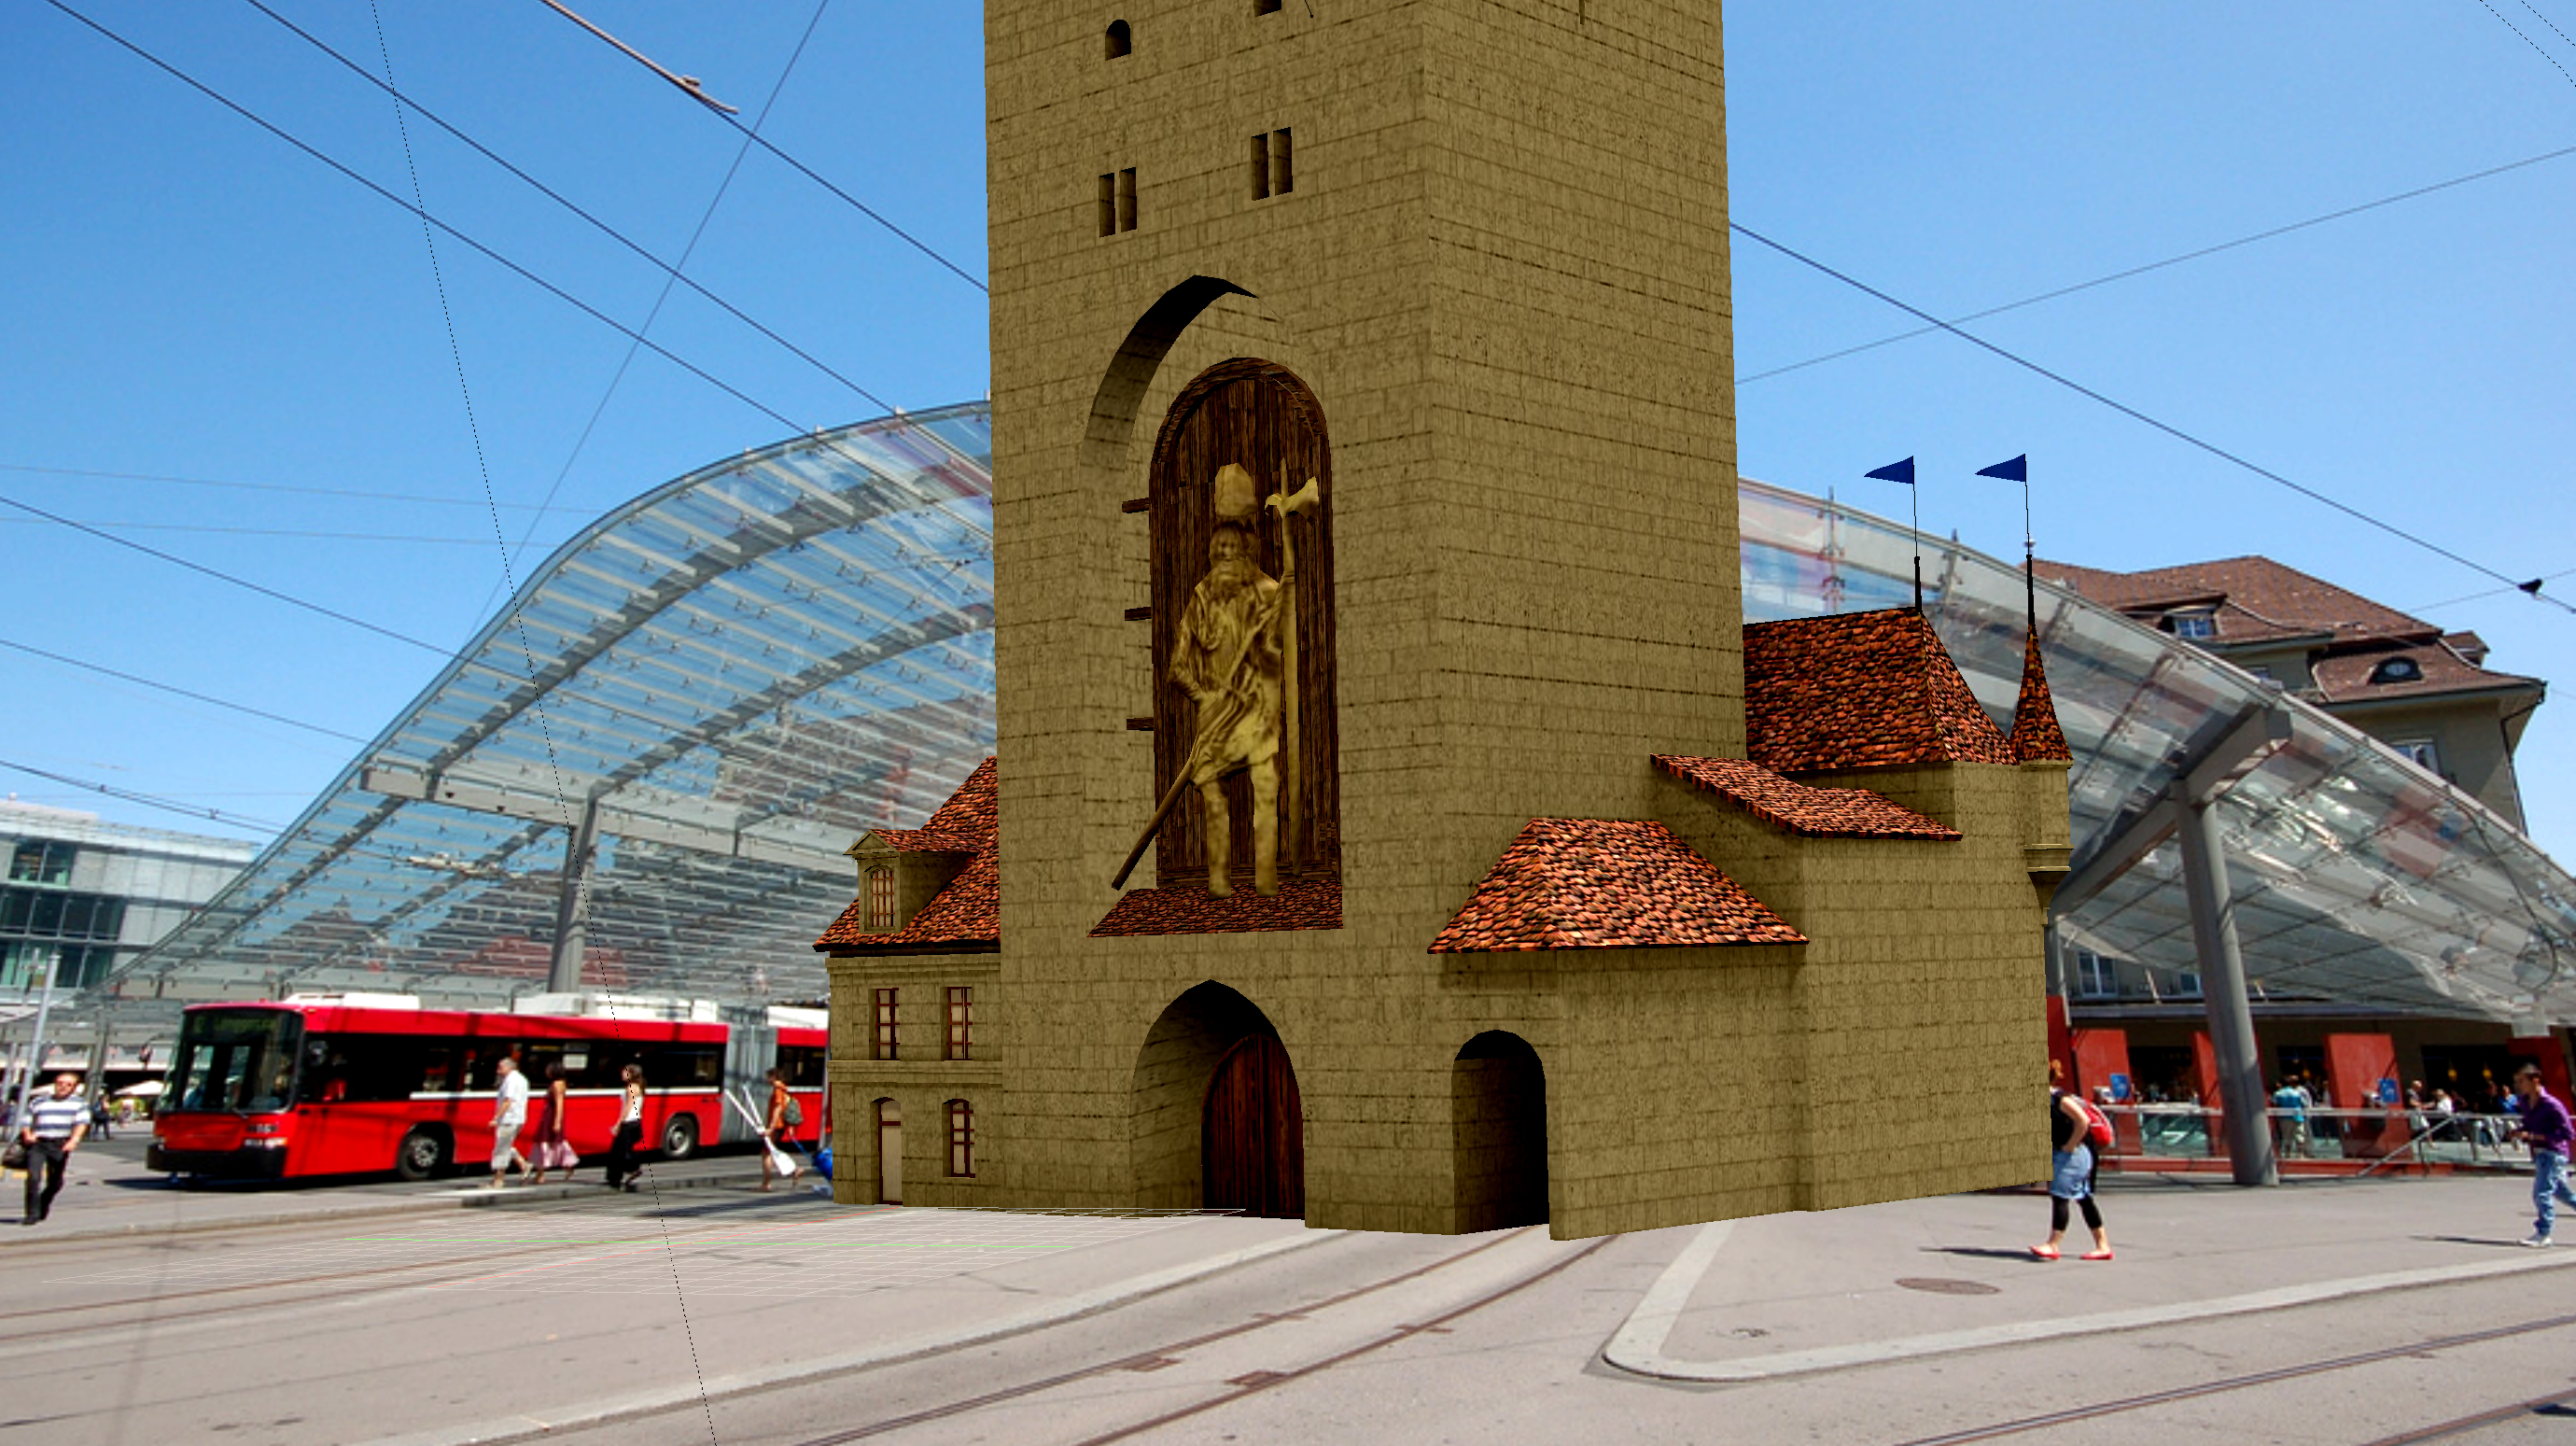
\includegraphics[width=1.0\textwidth]{img/christoffeltower.png}
  \end{center}
	\caption{Christoffeltower with AR}\label{fig:christoffeltower}
\end{figure}
One problem of this idea is that we don't know what kind of device a possible viewer will use. Therefore it is not possible to use calibration data of a predefined camera type. It must be possible to calibrate the camera just in place. This is what this project tries to address. The goal is to calibrate a camera based on a pre-generated point cloud.\\\\
The following sections will explain why camera calibration is necessary and what camera calibration means.

\section{Camera Calibration}\label{sec:calibration}
Camera calibration is necessary to find a model that expresses the properties of a camera. Properties of a camera are:

\begin{itemize}
	\item Focal length of the camera lense
	\item Principal point on the camera sensor, where the z axis of the cameras coordinate system goes through.
	\item Distortion of the camera lense
	\item Size of a pixel
\end{itemize}

If we once know the camera model and the camera position, we can project virtual objects into a real world image. Figure \ref{fig:model} shows an image of a checkerboard where we project a virtual cube onto. One camera model in this image took distortion into account while the other one ignored it.
\begin{figure}[H]
  \begin{center}
		\includegraphics[width=1.0\textwidth]{img/model.png}
  \end{center}
	\caption{Applied camera model with (red) and without(green) distortion}\label{fig:model}
\end{figure}

\section{Goals}
We should write a program that takes a 3D point cloud and its corresponding 2D points as inputs and calculates the camera model. The tasks for this project are:
\begin{itemize}
\item Search existing solutions
\item Get used to the topics SLAM, AR, 3D and 2D coordinates
\item Choose a programming environment (Python, Matlab)
\item Implement a proof of concept with synthetic data
\item Implement a proof of concept with real-world data
\end{itemize}

\section{Timetable}

The project was planned to end on beginning of June because the exams are held in mid-June. The evaluation started well and finished in the given time. Unfortunately, the problems started with the implementation. The first algorithms worked purely because only non-linear optimization was used. Debugging and searching new approaches took more time than expected. Additional because of changing the employer it was not possible to invest the planned time for the project during April, May and June. Fortunately, the latest date for submitting this project is mid-August therefore it was possible to extend the time frame. The planned timeline is shown in figure \ref{fig:timeline_should} and the final timeline is show in figure \ref{fig:timeline_is}.
\begin{figure}[H]
	\includegraphics[width=1.0\textwidth]{img/timeline_should.png}
	\caption{Planned timeline}\label{fig:timeline_should}
\end{figure}

\begin{figure}[H]
	\includegraphics[width=1.0\textwidth]{img/timeline_is.png}
	\caption{Final timeline}\label{fig:timeline_is}
\end{figure}


\chapter{Evaluation}

As a first task we study some existing solutions to similar problems and we analyze different tools to gain an overview about the topic.

\section{Existing methods}

There are several papers about camera calibration available. However, most of them are improvements or additions to the checkerboard calibration \ref{sec:checkerboard}.

\subsection{Checkerboard}\label{sec:checkerboard}
The most famous variant for camera calibration is the checkerboard approach \cite{Zhang}. For this approach one must take photos of a checkerboard. The algorithm then performs the following tasks:
\begin{enumerate}
  \item Search the checkerboard inner corners
  \item Find an approximation of the intrinsic matrix
  \item Find an approximation of the extrinsic matrix
  \item Solve the non-linear camera model by minimizing the re-projection error with Levenberg-Marquardt
\end{enumerate}

\subsection{Self-calibration with planar scene}
In comparison to the checkerboard calibration this approach doesn't need a checkerboard. It uses the same technique as checkerboard calibration but instead of using a known image any planar image can be used for calibration \cite{selfcalib}. The algorithm tries to estimate the camera model by doing a bundle adjustment over several images. In comparison to the checkerboard calibration this is more computational expensive and requires more images for doing the calibration.

\subsection{Decision}
Because the checkerboard calibration is widely used and well documented, some ideas were taken from this approach. We don't have a checkerboard available but a 3D cloud instead. We will see that because we have a 3D cloud available we only need one image to estimate the camera parameters. Checkerboard calibration needs at least two images \cite{Zhang} but more will improve the result. The self calibrating approach is interesting but it wouldn't profit from the 3D point cloud. Further it would requires a planar image. In our case we don't have such an image available.

\section{Tools}
To do experiments and to implement a proof of concept, we need the right tool available. Here we inspect Matlab and Python. Both are widely used in computer vision today.

\subsection{Matlab}
Matlab has a powerful imaging toolbox. Besides that Matlab also has a lot of powerful tools to plot images, graphs etc. Matlab is a proprietary product of Mathworks. Matlab is available for all major operating systems. It provides all we need out of the box with the ``Image Processing Toolbox''.

\subsection{Python}
Python does not provide that many powerful tools out of the box as Matlab. However, through additional libraries it can become as powerful as Matlab. Python is developed as open source software and is available for all major operating systems.\\
We require the following additional libraries to have similar functionality as Matlab:
\begin{itemize}
  \item Scipy
    \subitem Adds mathematically functions like Levenberg-Marquardt or linear least squares
  \item Numpy
		\subitem Is a powerful framework for handling matrices (used by Scipy and OpenCV)
  \item OpenCV
		\subitem Adds image processing and computer vision (CV) features
  \item Matplotlib
    \subitem Adds some powerful visualisation utilities
\end{itemize}

\subsection{Decision}
Because Python has a fast growing community and because we can use OpenCV as CV-toolkit, we use Python as programing language/toolbox. It should be easy to port code written in Python/OpenCV to C++/OpenCV if required.

\chapter{Implementation}\label{chap:implementation}

In this chapter we see the different steps required to calibrate a camera. We start with basics about optimization, will understand the camera model, learn how to calibrate a camera and finally see a resulting algorithm.

\section{Optimization}
What we will see later is that we require an optimization algorithm to fit a model to an actual camera. We will use two different optimization algorithms. One is linear least squares which is an optimization algorithm that minimises linear mean squares problems. The second algorithm we will use is Levenberg-Marquardt to solve nonlinear least squares problems. This section describes the differences between these algorithms and which algorithm we should use for which problem.

\subsection{Linear least squares}
Assume we have a problem shown in the form of equation \ref{eq:least_squares_example1}.
\begin{equation}\label{eq:least_squares_example1}
  A*X=B=\begin{pmatrix}
    a_{11} & a_{12} \\
    a_{21} & a_{22}
  \end{pmatrix}*
  \begin{pmatrix}
    x_1 \\
    x_2
  \end{pmatrix}=
  \begin{pmatrix}
    b_1 \\
    b_2
  \end{pmatrix}
\end{equation}
Where:
\begin{align*}
  a		  &: \text{known input values}\\
  x	  	&: \text{unkonwns}\\
  b		  &: \text{known output values}
\end{align*}
We try to find the variable x. This is an easy doable task by inverting Matrix A and multiply the inverse with B. This will give us the unknown matrix X ($x_1,x_2$). We assume here that matrix A is nonsingular. Let us assume we have more equations than unknowns which is a common use case in reality. We will then have something like in equation \ref{eq:least_squares_example2}. This example isn't solvable by inverting matrix A. Instead we need a new algorithm called linear least squares \ref{eq:least_squares_algorithm}. This algorithm tries to minimize the squared error of the equation. For more details on why this algorithm works see \cite{Hayes}. Libraries that implement these algorithms can often do a pseudo-inverse instead of a simple inverse in case that a matrix is singular. Such an implementation is e.g. pinv of Numpy \cite{pinv}.

\begin{equation}\label{eq:least_squares_example2}
  A*X=B=\begin{pmatrix}
    a_{11} & a_{12} \\
    a_{21} & a_{22} \\
    a_{31} & a_{32} \\
    a_{41} & a_{42}
  \end{pmatrix}*
  \begin{pmatrix}
    x_1 \\
    x_2
  \end{pmatrix}=
  \begin{pmatrix}
    b_1 \\
    b_2 \\
    b_3 \\
    b_4
  \end{pmatrix}
\end{equation}

\begin{equation}\label{eq:least_squares_algorithm}
  X=(A^H*A)^{-1}*A^H*B 
\end{equation}

An advantage of using a linear solver for the least squares problem is that it will find the global minimum. It is also computationally faster for problems with low to medium amount of unknowns (1-100). However, as the name states it can only solve problems where the unknowns are linear dependent.

\subsection{Gradient-Descent}

Non-linear problems are much harder to solve. Algorithms for this kind of problem can't guarantee to find the global optimum if the problems are non-convex. One of the most common non-linear solver is Gradient-Descent. Gradient-Descent is an iterative algorithm which calculates the gradient at point x and then takes a step in the opposite direction of the gradient for minimizing a problem (see Figure \ref{fig:gradient_descent}). Gradient-Descent works iteratively and uses equation \ref{eq:gradient_descent} to take a step in direction of the minimum.

\begin{figure}[H]
  \begin{center}
    \includegraphics[width=0.5\textwidth]{img/gradient_descent.png}
  \end{center}
    \caption{Gradient-Descent}\label{fig:gradient_descent}
\end{figure}

\begin{equation}\label{eq:gradient_descent}
  X_{n+1}=X_n-\theta*\Delta f(X_n)
\end{equation}
Where:
\begin{align*}
  X		      &: \text{variables}\\
  \Delta f  &: \text{derivation of function f}\\
  \theta    &: \text{step size}
\end{align*}

Gradient-Decent is easy to implement and works well on most non-linear optimization problems. Gradient-Descent can be slow if the gradient is vanishing.

\subsection{Gauss-Newton}
The Newton optimization algorithm is an algorithm that assumes a problem is approximately quadratic near the optimal solution. It fits a polynomial at the current location, derives it and jumps to the position where the derivation of this polynomial is zero (Figure \ref{fig:newton}a). If the problem is quadratic near the optimal solution, this algorithm converges faster than gradient descent.

\begin{figure}[H]
	\centering
	\subfloat[Idea of Newton optimization\cite{newton_image}]{\includegraphics[width=0.4\textwidth]{img/newton.png}}
	\qquad
	\subfloat[Not converging in step 3]{\includegraphics[width=0.4\textwidth]{img/gn_converge.png}}
	\caption{Newton algorithm}
	\label{fig:newton}
\end{figure}

Gauss-Newton, only works to minimize a sum of squared values while classic Newton works on all problems. However, Gauss-Newton has the advantage of being computational faster \cite{gauss_newton}. It doesn't compute the Hessian matrix (second derivate). Gauss-Newton also works iteratively and uses update equation \ref{eq:gauss_newton}. 

\begin{equation}\label{eq:gauss_newton}
  X_{n+1} = X_n - (J_n^T*J_n)^{-1}*J_n*e_n
\end{equation}
Where:
\begin{align*}
  X		  &: \text{parameters to tune}\\
  n		  &: \text{step}\\
	J		  &: \text{Jacobian matrix \cite{Jacobian}}\\
  e  	  &: \text{error y-ŷ}
\end{align*}

Newton/Gauss-Newton can not guarantee to converge if the problem is not quadratic near the optimal solution as shown in Figure \ref{fig:newton}b. In this image the problem is nearly linear near the optimum therefore it can't find the solution.

\subsection{Levenberg-Marquardt}
For this project we choose Levenberg-Marquardt as non-linear optimization algorithm. Zhang proposed this who first described the checkerboard calibration \cite{Zhang}. Levenberg-Marquardt uses Gauss-Newton which makes it fast to converge but can move to Gradient-Descent if Gauss-Newton isn't converging. This makes Levenberg-Marquardt more robust than Gauss-Newton but makes it still faster than Gradient-Descent. Equation \ref{eq:levenberg_marquardt} shows the update equation for the parameters. \mu\ is the tuning parameter which will increase the influence of Gradient-Descent. If \mu\ is tiny (close to 0) then Levenberg-Marquardt only uses Gauss-Newton. If \mu\ is huge, then it uses only Gradient-Descent for optimization. The implementation of Levenberg-Marquardt can update \mu\ during optimization. If the error increases from step to step, the algorithm decreases the influence of Gauss-Newton and increases the influence of Gradient-Descent. It will therefore converge even if the problem is not quadratic near the optimal solution.

\begin{equation}\label{eq:levenberg_marquardt}
  X_{n+1} = X_n - (J_n^T*J_n + \mu*I)^{-1}*J_n*e_n
\end{equation}
Where:
\begin{align*}
  x		  &: \text{Parameters to tune}\\
  n		  &: \text{Step}\\
  J		  &: \text{Jacobian}\\
  \mu	  &: \text{Learning coefficient for Gradient-Descent}\\
  I     &: \text{Identity matrix}\\
  e  	  &: \text{The error y-ŷ}
\end{align*}

\section{Camera model}
The camera model expresses how any point in the three-dimensional space is projected onto a two-dimensional image. As a first approximation it assumes that all rays are going trough one point. This is called the pinhole camera model \ref{fig:projection}a. Given this assumption we can describe the projection of a 3D point onto a 2D image as shown in equation \ref{eq:cm}. We calculate the pixel location $x,y$ on the image by normalizing with $s$ as show in equation \ref{eq:cm_normalized} \cite{rvc}.
\begin{equation}\label{eq:cm}
  \begin{pmatrix}
		f_x & \gamma & c_x \\
		0 & f_y & c_y \\
		0 & 0 & 1 \\
	\end{pmatrix}*
	\begin{pmatrix}
		r_{00} & r_{01} & r_{02} & t_x \\
		r_{10} & r_{11} & r_{12} & t_y \\
		r_{20} & r_{21} & r_{22} & t_z \\
	\end{pmatrix}
	\begin{pmatrix}
		X \\
		Y \\
		Z \\
		1
	\end{pmatrix}=
	\begin{pmatrix}
		u \\
		v \\
		s
  \end{pmatrix}
\end{equation}
\begin{equation}\label{eq:cm_normalized}
	\begin{pmatrix}
		x \\
		y
	\end{pmatrix}=
	\begin{pmatrix}
		u/s \\
		v/s 
  \end{pmatrix}
\end{equation}

Where:
\begin{align*}
  X,Y,Z			&: \text{point in the 3D world}\\
	u,v,s	   	&: \text{point in 2D image not normalize}\\
	x,y				&: \text{point in 2D image normalized with s}\\
	f_x,f_y  	&: \text{focal length of the camera}\\
  c_x,c_y  	&: \text{principal point}\\
  t_x,t_y,t_z	&: \text{location of the camera}\\
  r_{ij}	&: \text{part of the rotation matrix}
\end{align*}

We can describe the intuition as follows. A Point (X,Y,Z) is projected onto an image sensor (u/s,v/s) by the multiplication of the intrinsic times the extrinsic matrix. The extrinsic matrix describes where the pinhole of the camera is located in the three dimensional space. The intrinsic camera matrix describes how the camera is constructed. For example, in figure \ref{fig:projection}b we translate and rotate a point $p_i$ with the extrinsic matrix so we can describe its coordinates with the pinhole as origin. Further we transform the point with the intrinsic camera matrix onto the image sensor.\\
\em
Note:\\
In chapter \ref{sec:cam_calib} we said we also need to know the pixel size. This is true but will not appear directly in the camera model. The parameters fx and fy who are sizes in meters are expressed in pixels. They therefore include the information about pixel size.
\normalfont

\begin{figure}[H]
	\centering
	\subfloat[Pinhole model]{\includegraphics[width=0.5\textwidth]{img/pinhole_camera_model.png}}
	\subfloat[3D point to 2D point]{\includegraphics[width=0.5\textwidth]{img/pnp.jpg}}
	\caption{Image projection}\label{fig:projection}
\end{figure}

When calibrating a camera we are interested in the intrinsic matrix because it will be constant over time for a specific camera. Additional to the intrinsic matrix a real world lense will have distortion. A lense will not map a point perfectly onto an image plane \cite{rvc}. It will misplace an image point non-linear the further away a pixel is from the principal point (cx,cy). We can see how distortion affects an image point in equation \ref{eq:dist} and equation \ref{eq:pdist}.

\begin{equation}\label{eq:dist}
	\begin{pmatrix}\gamma_{x} \\
	  \gamma_{y}
	\end{pmatrix}=\begin{pmatrix}
	  x(k_1r^2+k_2r^4+k_3r^6)\\
	  y(k_1r^2+k_2r^4+k_3r^6)
	\end{pmatrix}+\begin{pmatrix}
	  2p_1xy+p_2(r^2+2x^2)\\
	  p_1(r^2+2y^2)+2p_2xy
	\end{pmatrix}
\end{equation}
\begin{equation}\label{eq:pdist}
\begin{pmatrix}x'\\y'\end{pmatrix}=\begin{pmatrix}
x\\y\end{pmatrix}+\begin{pmatrix}\gamma_{x}\\\gamma_{y}\end{pmatrix}
\end{equation}
\begin{equation}\label{eq:radius}
	r = \sqrt{\left(\frac{x-c_x}{f_x}\right)^2+\left(\frac{y-c_y}{f_y}\right)^2}
\end{equation}
Where:
\begin{align*}
  k_{i}					&: \text{radial distortion}\\
  p_{i}					&: \text{tangential distortion}\\
	\gamma_{x,y}	&: \text{summed distortion}\\
  x',y'					&: \text{distorted image points}\\
	r							&: \text{distance from principal component equation \ref{eq:radius}} \\
	f_x,f_y				&: \text{focal lenght}
\end{align*}

By doing camera calibration we try to find a model which maps the 3D points onto a 2D image. The image calculated by the model must be as close as possible to the real image. In the next section we will see how a model will be optimized until it fits the real camera.

\section{Camera calibration}\label{sec:cam_calib}
This section describes how we use the camera model to calibrate a camera. This means how we fit a model to the real camera.

\subsection{Estimate the projection matrix}\label{sec:est_proj}
The camera model that includes distortion is a non-linear model. The reason for that is that several parameters are also available in squared form if we merge the distortion model with the extrinsic and intrinsic model. Therefore, we need to do non-linear optimization to find the real camera model. However, non-linear optimization can only find local optima. Therefore we require a good initial guess of where we start the optimization. We assume the distortion is small. We therefore ignore distortion in a first step. Our task is to find the $p_{ij}$ values in equation \ref{eq:projection}. The projection matrix P (containing $p_{nn}$) is a multiplication of the intrinsic times the extrinsic matrix.\\
\em
Note:\\
The assumption that distortion is small holds for regular lenses but not for fisheye lenses. We are focusing on regular ones for this project.
\normalfont

\begin{equation}\label{eq:projection}
	\begin{pmatrix}p_{11} & p_{12} & p_{13} & p_{14}\\
		p_{21} & p_{22} & p_{23} & p_{24}\\
		p_{31} & p_{32} & p_{33} & p_{34}\\
	\end{pmatrix}*
	\begin{pmatrix}
		X \\
		Y \\
		Z \\
		1
	\end{pmatrix}=
	\begin{pmatrix}
		u \\
		v \\
		s
  \end{pmatrix}
\end{equation}
Where:
\begin{align*}
	p_{ij}		&: \text{Unknown camera projection values of projection matrix P}\\
	X,Y,Z			&: \text{3D Point}\\
	u,v,s			&: \text{2D Point}\\
\end{align*}

We can rewrite equation \ref{eq:projection} as shown in equation \ref{eq:projection_flat}. We don't know u and v directly. We only have the pixel position which is $x=u/s, y=v/s, 1$. There is no way to estimate s. We know that s equals to the third row of equation \ref{eq:projection_flat}. If we multiply x and y by the third row, the equation will still hold (equation \ref{eq:projection_flat_s}). As a side effect we can remove the third row because the left and right side are equal which always holds. We finally have two equation per image point. Another trick we use is to set $p_{34}$ to 1. This makes the Z position of the camera the norm for the other unknowns. Because of this change the trivial solution where every unknown is zero disappears. We can solve the final equation \ref{eq:projection_flat_red} for all unknowns $p_{ij}$ with linear least square.

% Make sure we can have the whole column matrix (normally a line break will follow after 10 columns)
\setcounter{MaxMatrixCols}{15}
\begin{equation}\label{eq:projection_flat}
	\begin{pmatrix}
		X & Y & Z & 1 & 0 & 0 & 0 & 0 & 0 & 0 & 0 & 0\\
		0 & 0 & 0 & 0 & X & Y & Z & 1 & 0 & 0 & 0 & 0\\
		0 & 0 & 0 & 0 & 0 & 0 & 0 & 0 & X & Y & Z & 1\\
	\end{pmatrix}
	\begin{pmatrix}p_{00}\\
		p_{11}\\
		p_{12}\\
		p_{13}\\
		p_{14}\\
		p_{21}\\
		p_{22}\\
		p_{22}\\
		p_{23}\\
		p_{31}\\
		p_{32}\\
		p_{33}\\
		p_{34} \\
	\end{pmatrix}=
	\begin{pmatrix}u\\
		v\\
		s\\
	\end{pmatrix}
\end{equation}

\begin{equation}\label{eq:projection_flat_s}
	\begin{pmatrix}u\\
		v\\
		s\\
	\end{pmatrix}=\begin{pmatrix}
		x*(X*p_{31}+Y*p_{32}+Z*p_{33}+p_{34})\\
		y*(X*p_{31}+Y*p_{32}+Z*p_{33}+p_{34})\\
		1*(X*p_{31}+Y*p_{32}+Z*p_{33}+p_{34})
	\end{pmatrix}
\end{equation}


\begin{equation}\label{eq:projection_flat_red}
	\begin{pmatrix}
		X & Y & Z & 1 & 0 & 0 & 0 & 0 & -uX & -uY & -uZ\\
		0 & 0 & 0 & 0 & X & Y & Z & 1 & -vX & -vY & -vZ
	\end{pmatrix}
	\begin{pmatrix}
		p'_{00}\\
		p'_{11}\\
		p'_{12}\\
		p'_{13}\\
		p'_{14}\\
		p'_{21}\\
		p'_{22}\\
		p'_{23}\\
		p'_{24}\\
		p'_{31}\\
		p'_{32}\\
		p'_{33}
	\end{pmatrix}=
	\begin{pmatrix}x\\
		y\\
	\end{pmatrix}
\end{equation}
Where:
\begin{align*}
	p_{ij}		&: \text{unknown camera projection values}\\
	p'_{ij}		&: \text{same as c but normalized to $p_{34}$}\\
	X,Y,Z			&: \text{3D Point}\\
	u,v,s			&: \text{2D Point with scale factor s}\\
	x,y				&: \text{2D Point normalize to s=1}\\
\end{align*}

We miss one last step. We set $p_{34}$ to 1 to get rid of the trivial solution where all $p_{ij}$ are zero. We now have to find the right value for $p_{34}$. If we calculate the intrinsic times the extrinsic matrix we end up in equation \ref{eq:ext_int}. We focus on the third row. We know that the norm of a column of a rotation matrix must be one. The reason for this is that a rotation matrix will never change the length of a vector. Therefore, $h=\sqrt{r_{31}^2+r_{32}^2+r_{33}^2}$ must be one \cite{Wu}. Because we normalized tz to one, this assumption does not hold for our solution. The camera distance $t_z$ will therefore be $1*1/h$. To correct the projection matrix we can multiply the matrix with $1/h$ (equation \ref{eq:ext_int_scaled}).

\begin{equation}\label{eq:ext_int}
	P=
	\begin{pmatrix}
		f_xr_{11}+p_xr_{31} & f_xr_{12}+p_xr_{32} & f_xr_{13}+p_xr_{33} & f_xt_x+p_xt_z\\
		f_yr_{21}+p_yr_{31} & f_yr_{22}+p_yr_{32} & f_yr_{23}+p_yr_{33} & f_yt_y+p_yt_z\\
		r_{31} & r_{32} & r_{33} & t_z
	\end{pmatrix}
\end{equation}

\begin{equation}\label{eq:ext_int_scaled}
	P=1/h
	\begin{pmatrix}
		p'_{11} & p'_{12} & p'_{13} & p'_{14}\\
		p'_{21} & p'_{22} & p'_{23} & p'_{24}\\
		p'_{31} & p'_{32} & p'_{33} & 1\\
	\end{pmatrix}
\end{equation}

Where:
\begin{align*}
	P					&: \text{projection matrix}\\
	p_{ij}'		&: \text{projection matrix found with $t_z=1$}\\
	f_x,f_y		&: \text{focal length}\\
	c_x,c_y		&: \text{principal point}\\
	r_{ij}		&: \text{Parameters of rotation matrix}\\
	t_{x,y,z}	&: \text{location of the camera}\\
	h					&: \text{scaling inverse $tz=1/\sqrt{r_{31}^{'2}+r_{32}^{'2}+r_{33}^{'2}}$}
\end{align*}


After we found the unknowns, we have a first approximation of the projection matrix. In the next step we need to decompose this projection matrix into the intrinsic and extrinsic matrix.\\

\subsection{Matrix decomposition}\label{sec:matrix_dec}
We can decompose any rectangular matrix into an upper triangular matrix times a rectangular matrix as shown in \ref{eq:uptriang}. In this equation the intrinsic matrix equals matrix R ($r_{ij}$), the extrinsic matrix equals matrix Q ($q_{ij}$) and the projection matrix equals matrix M ($m_{ij}$).
\begin{equation}\label{eq:uptriang}
	\begin{pmatrix}
		r_{11} & r_{12} & r_{13}\\
		0 & r_{22} & r_{23}\\
		0 & 0 & r_{33}
	\end{pmatrix}
	\begin{pmatrix}
		q_{11} & q_{12} & q_{13}\\
		q_{21} & q_{22} & q_{23}\\
		q_{31} & q_{32} & q_{33}
	\end{pmatrix}=
	\begin{pmatrix}
		m_{11} & m_{12} & m_{13}\\
		m_{21} & m_{22} & m_{23}\\
		m_{31} & m_{32} & m_{33}
	\end{pmatrix}
\end{equation}

This decomposition is called RQ-decomposition \cite{qr_decomposition}. Most mathematic libraries don't offer the RQ-decomposition but a QR-decomposition which is a relative. In this project we use the following algorithm \cite{rq_stack} for QR/RQ conversion:
\begin{enumerate}
	\item Compute $A^{*}=P*A$ (Where P = equation \ref{eq:qr_p})
	\item Compute decomposition of $A^{*T}=Q^*R^*$
	\item Set $Q=PQ^{*T}$ (i.e. reverse rows of $Q^{*T}$, note that Q is orthogonal)
	\item Set $R=PR^{*T}P$
\end{enumerate}

\begin{equation}\label{eq:qr_p}
	P=\begin{pmatrix}
		0 & 0 & 1\\
		0 & 1 & 0\\
		1 & 0 & 0
	\end{pmatrix}
\end{equation}
\em
Note:\\
There is an additional parameter $r_{12}$ which we don't use in the camera model. In theory this value should converge to zero. In reality this value will be small but more than zero. For non-linear estimation we set $r_{12}$ to zero. The non-linear optimization of the following section will anyway optimize the whole model again.
\normalfont

\subsection{Non-Linear estimation}\label{sec:nonlinear_est}
Until now we ignored the non-linear distortion. We took a simple linear model and optimized it to find the intrinsic camera matrix. This matrix can be used as initial guess for optimizing the non-linear model. For the non-linear optimization we calculate the re-projection error of each point as shown in equation \ref{eq:reprojecterr}. 
\begin{equation}\label{eq:reprojecterr}
	e=\sum\limits_{i=1}^n(x_{should}-x_{is})^2 +(y_{should}-y_{is})^2
\end{equation}
Where:
\begin{align*}
	e												&: \text{re-projection error}\\
	x_{should},y_{should}		&: \text{the real x and y position of the point}\\
	x_{is},y_{is}						&: \text{the x and y position when applying the camera model}\\
\end{align*}

In some resources we find that it is possible to calculate a first guess for the distortion parameters with a linear model as well. In theory this is true with equation \ref{eq:distortion_lin}.  However, because the intrinsic and extrinsic camera matrix is an approximation the linear least squared solution for the distortion will be wrong. Instead, a good initial estimation of the distortion parameters is to assume all parameters are zero. The reason why zero is a good guess is because we assumed that during linear optimization. After that we can optimize the whole camera model with Levenberg-Marquardt by minimizing the re-projection error of equation \ref{eq:reprojecterr}. We calculate the re-projection error during each iteration of Levenberg-Marquardt for every point. The Jacobian matrix is calculated with discrete values because we don't have a Jacobian of our model available. Levenberg-Marquardt will now minimize the squared sum of all re-projection errors.

\begin{equation}\label{eq:distortion_lin}
	\begin{pmatrix}
		f_x\\
		f_y
	\end{pmatrix}.*
	\begin{pmatrix}
		xr^2 & xr^4 & xr^6 & 2xy & r^2+2x^2 \\
		yr^2 & yr^4 & yr^6 & r^2+2y^2 & 2xy
	\end{pmatrix}
	\begin{pmatrix}
		k1\\k2\\k3\\p1\\p2
	\end{pmatrix}=
	\begin{pmatrix}
		u_{should}-u_{est}\\
		v_{should}-v_{est}
	\end{pmatrix}
\end{equation}
Where:
\begin{align*}
  f_x/f_y		&: \text{focal length}\\
	x,y				&: \text{Position on the sensor measured from principal point}\\
	r					&: \text{Radius measured from principal point}\\
	k1,k2,k3	&: \text{Radial distortion}\\
	p1,p2			&: \text{Tangential distortion}\\
	.*				&: \text{Element wise matrix multiplication}
\end{align*}

Until now we didn't assume we have misleading data available in our dataset. In reality there are often outliers in a dataset which should be removed. In the next section we will see how this can be done.

\subsection{Outlier Detection}\label{sec:outliers}
The described approach so far works well if there are no outliers in the dataset. This is true for synthetic data but not for real world data. Therefore an algorithm is needed to detect outliers. For this project an algorithm similar to RANSAC \cite{ransac} is used. Instead of calculating the projection matrix \ref{eq:projection} once, the calculation is done iteratively with a reduced and randomized dataset. The estimation that fits the data best will be used for further calculation. Outliers that have a huge re-projection error will be removed from the dataset. The algorithm used can be described as follows:
\begin{enumerate}
	\item Get a random subset of 10 data points
	\item Calculate the projection matrix as described in section \ref{sec:est_proj}
	\item Calculate the 2D projection based on the estimated camera model
	\item Calculate the distance of each point to where it should be
	\item Count the point as hit if it is within a radius of 3 pixels
	\item Repeat steps 1-5 n times, take the model with the most hits
	\item Remove all points that do not count as hit from the dataset
\end{enumerate}

In this project n was chosen to be 2000. Increasing this value will make the algorithm more robust but also slower.

\subsection{Final algorithm}
Now that we have everything in place we can put together the final algorithm as follows:
\begin{enumerate}
	\item Take a randomized reduced set of data from the dataset \ref{sec:outliers}
	\item Calculate the projection matrix with linear least squares \ref{sec:est_proj}
	\item Calculate the projection of each point
	\item Detect outliers \ref{sec:outliers}
	\item Repeat steps 1-4 n times
	\item Do the matrix decomposition \ref{sec:matrix_dec} to find the intrinsic matrix
	\item Do non-linear estimation \ref{sec:nonlinear_est} to optimize the camera model with distortion
\end{enumerate}

The final output will be the intrinsic matrix and the five distortion parameters $k_i$ + $p_i$. As a side effect we also get the extrinsic camera matrix.

\section{Point cloud}
So far we ignored how we find 3D and 2D points for estimating the camera model. This step is not part of this project, however it is needed to generate a real world example. This section gives a small overview on how a 3D point cloud can be generated.\\
A point cloud is a collection of points within a 3-dimensional space. We know the position (x,y,z) of each point and its unique descriptor. The descriptor must be translation and rotation invariant. The cloud can be stored in a file or database for further use. We chose ORB2 monocular SLAM \cite{orbslam2} to generate this cloud because it is open source, good documented and well established. Monocular SLAM is chosen because its handling is easier than with other systems (e.g. stereo camera). ORB2 Slam performs simplified the following steps:
\begin{enumerate}
	\item Search distinctive points on the image e.g. corners
	\item Calculate an ORB descriptor around all distinctive points
	\item Find similar descriptors on the next image
	\item Calculate the rotations and translation between the two images
	\item Calculate the position of the camera
	\item Calculate the position of the points
\end{enumerate}
We store the position and the ORB descriptor of each point in a file to make the point cloud persistent.
This projects goal wasn't to generate a point cloud therefore we don't explain the algorithm and steps in more detail here. In theory any type of point cloud could be used as long as the 3D points can be matched against 2D points. The next section will describe how we find the corresponding 3D points on a 2D image.

\section{Point Matching}
To do camera calibration we need a set of 2D and 3D points. We need to know the position of a 2D point in an image and in the 3D world. The steps to find a set of 2D/3D points can be described as follows:
\begin{enumerate}
	\item Search distinctive points on the image e.g. corners
	\item Calculate an ORB descriptor around all distinctive points
	\item Match the ORB descriptors of the image with the ORB descriptors from the 3D point cloud using hamming distance
	\item Use the 2D/3D dataset for doing camera calibration
\end{enumerate}

This algorithm was used to implement the real world example.

\chapter{Result}

In this document we saw a technique on how camera calibration can be done with a pre-generated point cloud. It works well when the 3D cloud is reliable. The following sections show two tools that came out of this project as well as a modified version of ORB Slam 2.\\

The software written during this project is available on Github under the following link \url{https://github.com/eichenberger/camera-calibration}. To setup everything the following commands need to be executed (Linux):
\small
\lstset{language=bash}
\begin{lstlisting}
git clone git@github.com:eichenberger/camera-calibration.git
cd camera-calibration
python3 setup.py install

# For proof of concept
cd poc
python3 poc.py -h
# Example
python3 poc.py

# For camera calibration
cd src
python3 camera-calibration.py -h
# Example
python3 camera-calibration.py test2.map keyframes/keyframe_2.png
\end{lstlisting}
\normalsize

\section{Proof of concept}

To test the algorithm with synthetic data a proof of concept has been written. With the proof of concept we are able to simulate noise and outliers to see how the algorithm performs. Because we know the exact camera parameters we can calculate the distance from the estimated values to the real values. This distance is calculated and printed on the console. It serves as an indicator how well the estimation works.\\

From the estimated camera model we calculate a projection of the model. The image with the known model and the image with the estimated model will be plotted. Such an image is shown in figure \ref{fig:diff_img}. To make differences visible in the example, white noise was added before doing the estimation. Without noise the estimated model would match the real model without any visible difference.
\begin{figure}[H]
  \begin{center}
		\includegraphics[width=1.0\textwidth]{img/diff_img.png}
  \end{center}
	\caption{Comparison real (green) with estimated (red) model when image data is noisy}\label{fig:diff_img}
\end{figure}

\section{Real data}
Another application was written to show that the proof of concept would also work with real-world data. The application takes as input a 3D point cloud (ORB Slam 2) and an image. With this information it performs the following steps:
\begin{enumerate}
	\item Search ORB keypoints on the image
	\item Calculate ORB descriptor around each keypoint
	\item Match ORB descriptors with descriptors found in the point cloud with BFMatcher \cite{BFMatcher} based on Hamming distance
	\item Generate pairs of 3D and 2D points based on matches from the previous step
	\item Start camera calibration as described in section \ref{sec:cam_calib}
\end{enumerate}
To generate the point cloud we modified the ORB2\_SLAM open source implementation \cite{orbslam2_impl}. The modification allows us to export 3D points and their corresponding descriptor. It would also be possible to use SLProject to generate the point cloud.\\

An example output of camera-calibration.py which is part of this project is shown here:
\tiny
\begin{lstlisting}
Start camera calibration
Extract descriptors
Match keypoints
Optimize camera model
Found camera parameters:
        fx      fy      cx      cy      thetax  thetay  thetaz  tx      ty      tz      k1      k2      k3      p1      p2
values: 1318.89 1320.44 646.11  361.73  0.04    0.01    0.03    0.01    -0.0    -0.01   0.35    -2.78   8.12    -0.01   0.0
Exit program
\end{lstlisting}
Values from checkerboard calibration for the same camera:
\begin{lstlisting}
        fx      fy      cx      cy      k1      k2      k3      p1      p2
values: 1333    1333    629     362     0.31    -2.37   6.65    -0.0003 0.0002
\end{lstlisting}
This gives us an uncertainty per parameter of:
\begin{lstlisting}
        fx      fy      cx      cy      k1      k2      k3      p1      p2
diff:   1.05%   0.94%   2.72%   0.07%   12.90%  17.30%  12.32%  32.33% 100%
\end{lstlisting}
\normalsize
Besides the small distortion parameters the calibration works well. The uncertainties are there because of noise and inaccuracy in the point cloud. However, the camera model would work well for augmented reality. An example of an undistorted image with the estimated parameters is shown in figure \ref{fig:undistorted}. Please note that the point clouds available in the repository ``test.map'' and ``test2.map'' aren't accurate, therefore it can sometimes happen that the non-linear optimization converges into an invalid optima. Unfortunately there is no detection for this in the current implementation.

\begin{figure}[H]
  \begin{center}
		\includegraphics[width=1.0\textwidth]{img/calib_output.png}
  \end{center}
	\caption{Undistorted image after calibration with colored keypoints}\label{fig:undistorted}
\end{figure}

\section{ORB Slam 2}
For creating the 3D point we can use a modified version of ORB\_SLAM2. This version allows controlling and accessing ORB slam from Python. The modified version can be found in this repo \url{https://github.com/eichenberger/ORB\_SLAM2} under the branch se. Please note that the state of this project is unstable. It unfortunately needs some manual work to get a final python library. The modification won't be documented here further because it wasn't officially part of this project.

\section{Improvements}\label{sec:improvements}
The algorithm described in this document only shows the calibration process on a single image. This works well but isn't very robust. OpenCV in comparison uses several images for doing checkerboard calibration. With this approach it can detect when the non-linear optimization goes in wrong directions. OpenCV also does bundle adjustment over several images which reduces the influence of noise and increases the robustness. This methods could be used to improve our algorithm as well and to make it more robust against noise, outliers and converging into wrong solutions.\\
\em
Note:\\
If we try to add boundaries to the optimization algorithm by punishing values diverging from the initial guess we introduce new local optima. It can therefore happen that in this case Levenberg-Marquardt converges into a wrong optimum.
\normalfont

\listoffigures
 
\begin{thebibliography}{1}

  \bibitem{surf}
  Herbert Bay1, Tinne Tuytelaars2, and Luc Van Gool,
  \textit{SURF: Speeded Up Robust Features}
  http://www.vision.ee.ethz.ch/~surf/eccv06.pdf (09.07.2018)

  \bibitem{orbslam}
  Raul Mur-Artal, J. M. M. Montiel, Juan D. Tardos
  \textit{ORB-SLAM: a Versatile and Accurate Monocular SLAM System}
  arXiv:1502.00956v2

  \bibitem{orbslam2}
  Raul Mur-Artal, J. M. M. Montiel, Juan D. Tardos
  \textit{ORB-SLAM2: an Open-Source SLAM System for Monocular, Stereo and RGB-D Cameras}
	arXiv:1610.06475v2 

  \bibitem{orbslam2_impl}
  Raul Mur-Artal, J. M. M. Montiel, Juan D. Tardos
  \textit{ORB-SLAM2 Implemenation}
	https://github.com/raulmur/ORB\_SLAM2


  \bibitem{selfcalib}
  Daniel Herrera et al.
  \textit{Forget the checkerboard: practical self-calibration using a planar scene}
  doi:10.1109/WACV.2016.7477641

  \bibitem{Hayes}
  Monson H. Hayes,
  \textit{Statistical Digital Signal Processing And Modeling},
  Wiley, ISBN 0-47159431-8

  \bibitem{pinv}
  Numpy,
  \textit{scipy.linalg.pinv},
  Compute the (Moore-Penrose) pseudo-inverse of a matrix

  \bibitem{gauss_newton}
  Wikipedia,
  \textit{Gauss-Newton algorithm},
  https://en.wikipedia.org/wiki/Gauss\%E2\%80\%93Newton\_algorithm (08.07.2018)

  \bibitem{newton_image}
  http://fourier.eng.hmc.edu,
  \textit{Newton Ralphson Method}
  http://fourier.eng.hmc.edu/e176/lectures/NM/node20.html (09.07.2018)

  \bibitem{Zhang}
  Zhengyou Zhang,
  \textit{A Flexible New Technique for Camera Calibration}
  MSR-TR-98-71

	\bibitem{rvc}
	Peter Corke,
	\textit{Robotics, Vision and Control}
	Springer, ISBN 978-3-319-54413-7, chapter 11+12, page 319+

	\bibitem{qr_decomposition}
	William H. Press,
	\textit{Numerical Recipes 3rd Edition: The Art of Scientific Computing, p102-109} 
	Cambridge University Press, ISBN 0-52188068-8

	\bibitem{rq_stack}
	johnnycrab,
	\textit{rq-decomposition} 
	https://math.stackexchange.com/questions/1640695/rq-decomposition (10.07.2018)

	\bibitem{ransac}
	wikipedia,
	\textit{RANSAC}
	https://de.wikipedia.org/wiki/RANSAC-Algorithmus

	\bibitem{BFMatcher}
	OpenCV,
	\textit{Brute-force descriptor matcher}
	https://docs.opencv.org/3.1.0/d3/da1/classcv\_1\_1BFMatcher.html

	\bibitem{Jacobian}
	Wikipedia,
	\textit{Jacobian matrix}
	https://en.wikipedia.org/wiki/Jacobian\_matrix\_and\_determinant

	\bibitem{Wu}
	Ying Wu,
	\textit{Image Formation and Camera Calibration}
	http://users.eecs.northwestern.edu/~yingwu/teaching/EECS432/Notes/camera.pdf (19.08.2018), Electrical Engineering \& Computer Science Northwestern University Evanston

\end{thebibliography}


\end{document}
